%%% LaTeX Template: Article/Thesis/etc. with colored headings and special fonts
%%%
%%% Source: http://www.howtotex.com/
%%% Feel free to distribute this template, but please keep to referal to http://www.howtotex.com/ here.
%%% February 2011

%%%%% Preamble
\documentclass[10pt,a4paper]{article}

\usepackage[T1]{fontenc}
\usepackage[bitstream-charter]{mathdesign}
\usepackage{graphicx}

\usepackage[latin1]{inputenc}							% Input encoding
\usepackage{amsmath}									% Math

\usepackage{xcolor}
\definecolor{bl}{rgb}{0.0,0.2,0.6} 


\usepackage{sectsty}
%\usepackage[compact]{titlesec} 
\allsectionsfont{\color{bl}\scshape\selectfont}

%%%%% Definitions
% Define a new command that prints the title only
\makeatletter							% Begin definition
\def\printtitle{%						% Define command: \printtitle
    {\color{bl} \centering \huge \sc \textbf{\@title}\par}}		% Typesetting
\makeatother							% End definition

\title{Documentation of the code}

% Define a new command that prints the author(s) only
\makeatletter							% Begin definition
\def\printauthor{%					% Define command: \printauthor
    {\centering \@author}}				% Typesetting
\makeatother							% End definition

\author{%
	\vspace{20pt}
	Adolfo V\'azquez-Quesada and Marco Ellero\\
%	mail@mail.com \\
	\vspace{20pt}
	}

% Custom headers and footers
\usepackage{fancyhdr}
	\pagestyle{fancy}					% Enabling the custom headers/footers
\usepackage{lastpage}	
	% Header (empty)
	\lhead{}
	\chead{}
	\rhead{}
	% Footer (you may change this to your own needs)
	\lfoot{\footnotesize \texttt{Code without solvent}}
	\cfoot{}
	\rfoot{\footnotesize page \thepage\ of \pageref{LastPage}}	% "Page 1 of 2"
	\renewcommand{\headrulewidth}{0.0pt}
	\renewcommand{\footrulewidth}{0.4pt}

% Change the abstract environment
\usepackage[runin]{abstract}			% runin option for a run-in title
\setlength\absleftindent{30pt}		% left margin
\setlength\absrightindent{30pt}		% right margin
\abslabeldelim{\quad}						% 
\setlength{\abstitleskip}{-10pt}
\renewcommand{\abstractname}{}
\renewcommand{\abstracttextfont}{\color{bl} \small \slshape}	% slanted text


%%% Start of the document
\begin{document}
%%% Top of the page: Author, Title and Abstact
\printtitle 

\printauthor

%\begin{abstract}
%Documentation of  the code for simulating  concentrated suspensions of
%spherical particles in a bi-viscous fluid.
%\end{abstract}

%%% Start of the 'real' content of the article, using a two column layout
\section{Introduction}
In  this  paper, the  documentation  for  the  code used  to  simulate
concentrated spherical particles in a fluid, considering lubrication
and friction between particles is
presented. Rotations of the particles are considered.
For further details, the reader may refer to \cite{kumar2021}, for the
description of the dynamics with rotation, and \cite{ruiz2023}, for the
description of the friction model.

\section{The code}
The code is written in Fortran in an Object-Oriented Programming style
(see  \cite{decyk1996}). The  classes  (class*  files) are  programmed
using modules  and type definitions.   Each class has  its subroutines
(inc* files) included in its own files. The main program is written in
main.f90.

To compile  the code,  the gfortran program  must be  installed. Other
fortran compilers  can be used  if the  makefile files are  edited. To
compile the code  type the following in the shell  (within the program
directory):

\begin{verbatim} 
make

make link
\end{verbatim}

To run the program, modify the \emph{input} file and then type:

\begin{verbatim} 
./biviscous_suspension
\end{verbatim}

For a clean recompilation, first type:

\begin{verbatim} 
make clean
\end{verbatim}

The input variables  are read from the \emph{input} file.  In the next
section, the meaning of each variable in the input file is explained.

\subsection{Input Variables}
An input file can be found in the `src` directory. The meanings of the inputs are indicated below:
\begin{itemize}

\item \textbf{Nsteps}: Number of steps.

\item \textbf{dt}: Time step.

\item \textbf{explicit}: \texttt{.TRUE.} if the explicit scheme is used; \texttt{.FALSE.} if the semi-implicit scheme \cite{bian2014,vazquez2016a,vazquez2016b} is used.

\item \textbf{sweep\_tol}: Tolerance for the semi-implicit scheme \cite{bian2014,vazquez2016a,vazquez2016b}. Used only if \textbf{explicit} = \texttt{.FALSE.}.

\item \textbf{N\_sweep\_max}: Maximum allowed number of sweeps. Used only if \textbf{explicit} = \texttt{.FALSE.}.

\item \textbf{dim}: Number of dimensions ($2$ or $3$).

\item \textbf{L}: Box size ($2$ or $3$ real numbers, corresponding to the length in the $x$, $y$, and $z$ directions).

\item \textbf{eta0}: Shear viscosity $\eta_0$ of the solvent.

\item \textbf{eta1}: When the biviscous model is considered \cite{vazquez2016c}, \textbf{eta1} is the shear viscosity $\eta_1$ at high shear rates. Used only if \textbf{biviscous} = \texttt{.TRUE.}.

\item \textbf{gamma\_dot}: The imposed shear rate $\dot{\gamma}$.

\item \textbf{gamma\_dot\_critical}: In the case of a bi-viscous fluid, the critical shear rate.

\item \textbf{biviscous}: \texttt{.FALSE.} if the solvent is Newtonian; \texttt{.TRUE.} if it is biviscous.

\item \textbf{d\_bulk}: Distance (in units of $L_z$) from the walls where we consider as bulk.

\item \textbf{N}: Number of particles. Used only if \textbf{read\_pos} = \texttt{.FALSE.}.

\item \textbf{R}: Radius of particles.

\item \textbf{mass}: Mass of particles.

\item \textbf{read\_pos}: \texttt{.FALSE.} if the program generates the positions of the particles (only possible for low concentrations); \texttt{.TRUE.} if the positions of the particles are read from a file.

\item \textbf{file\_pos}: Route of the file to read the positions of the particles. Used only if \textbf{read\_pos} = \texttt{.TRUE.}.

\item \textbf{read\_vel}: \texttt{.TRUE.} if the velocities are read from a file; \texttt{.FALSE.} if the program generates the velocities of the particles. The velocity imposed initially on the particles corresponds to the velocity profile of shear rate $\dot{\gamma}$.

\item \textbf{file\_vel}: Route of the file to read the velocities of the particles. Used only if \textbf{read\_vel} = \texttt{.TRUE.}. If \textbf{read\_vel} = \texttt{.FALSE.}, all particle velocities are set to zero.

\item \textbf{rcut}: Cutoff radius for interactions between particles.

\item \textbf{rcut\_on}: Cut-on radius for interactions between particles.

\item \textbf{rlist}: Value greater than $1$ (and close to $1$) that allows calculation of the skin around \textbf{rcut} to find neighbors. The radius of the sphere to search for neighbors will be \textbf{rlist} $\times$ \textbf{rcut} (see the section \emph{The Verlet neighbor list} in \cite{allen1989}).

\item \textbf{tau}: The parameter $\tau$ of the repulsive force \cite{bian2014,vazquez2016a,vazquez2016b}.

\item \textbf{F0}: The parameter $F_0$ of the repulsive force \cite{bian2014,vazquez2016a,vazquez2016b}.

\item \textbf{fixed\_seed}: \texttt{.TRUE.} if the seed is selected by the user; \texttt{.FALSE.} if the seed is generated automatically.

\item \textbf{seed}: Seed for the random number generator. Used only if \textbf{fixed\_seed} = \texttt{.TRUE.}.

\item \textbf{dir\_output}: Route of the directory where the program will output data. If the directory does not exist, it will be created by the program.

\item \textbf{freq\_write}: Frequency to output all data except particle data.

\item \textbf{freq\_write\_part}: Frequency to output particle data.

\item Some variables are still without description. If you need clarification do not hesitate to contact us.

\end{itemize}

\subsection{Classes}

\begin{itemize}

\item \textbf{Class computational}: Defines the precision of the real numbers.

\item \textbf{Class input}: Class to read the input variables from a file.

\item \textbf{Class read input}: Class with general tools to read variables of many different types from files.

\item \textbf{Class system}: Contains all the necessary variables for the simulation.

\item \textbf{Class particle}: Class for particle objects.

\item \textbf{Class random}: Class for the random number generator.

\item \textbf{Class output}: Class for output files.

\item \textbf{Class cell}: Class for cell objects used to search for neighbors (see \cite{allen1989}).

\item \textbf{Class wall}: Class for wall objects.

\item \textbf{Class comp\_time}: Class for calculating computation times.

\item \textbf{Class files\_utilities}: Collection of several utilities to handle files.

\item \textbf{Class file}: Class for file objects.

\item \textbf{Class functions\_utilities}: Collection of utilities related to functions.

\end{itemize}

Aqu� est� el texto revisado en formato LaTeX:

\subsection{Key for Output Files}
\begin{itemize}

\item \emph{info.dat}: General information about the simulation. The meaning is self-explanatory.

\item \emph{input}: A copy of the input file.

\item \emph{comp\_time.dat}: File with data about the time taken by the code to perform tasks. The columns are:
  \begin{enumerate}
    \item Time step.
    \item Total computational time.
    \item Neighbour searching computational time.
    \item Semi-implicit scheme computational time.
    \item Velocity-Verlet computational time.
  \end{enumerate}

\item Initial positions file: If the initial positions have been read from a file, this file will be copied into the output directory.

\item Initial velocities file: If the initial velocities have been read from a file, this file will be copied into the output directory.

\item \emph{walls.dat}: File with data from walls. The columns in 3D are (in 2D, the columns are fewer):
  \begin{enumerate}
    \item Time step.
    \item $x$ force on the bottom wall.
    \item $y$ force on the bottom wall.
    \item $z$ force on the bottom wall.
    \item $x$ force on the top wall.
    \item $y$ force on the top wall.
    \item $z$ force on the top wall.
  \end{enumerate}

\item \emph{stress.dat}: File with the stress tensor $\boldsymbol{S}_{pp}$ calculated from the bulk. The columns in 3D are (in 2D, the columns are fewer):
  \begin{enumerate}
    \item Time step.
    \item $S_{pp}^{xx}$.
    \item $S_{pp}^{xy}$.
    \item $S_{pp}^{xz}$.
    \item $S_{pp}^{yx}$.
    \item $S_{pp}^{yy}$.
    \item $S_{pp}^{yz}$.
    \item $S_{pp}^{zx}$.
    \item $S_{pp}^{zy}$.
    \item $S_{pp}^{zz}$.
  \end{enumerate}

\item \emph{particles\ldots.dat}: Files with data about particles. The columns in 3D are (in 2D, the columns are fewer):
  \begin{enumerate}
    \item Particle identity (an integer).
    \item Particle $x$ position.
    \item Particle $y$ position.
    \item Particle $z$ position.
    \item Particle $x$ velocity.
    \item Particle $y$ velocity.
    \item Particle $z$ velocity.
    \item Particle radius.
  \end{enumerate}

\item \emph{shear\_rate.dat}: File with the calculated shear rate (which may be smaller than the input shear rate).
  \begin{enumerate}
    \item Time step.
    \item Calculated shear rate.
  \end{enumerate}

\end{itemize}

\subsection{Before Simulating}
To create the initial configuration of particles, the algorithm of the
code randomly fills the space with non-overlapping particles at random
positions. This  approach works well  for low concentrations,  but for
concentrated cases, it may not  achieve a valid configuration. In such
cases, the initial configuration should be provided by the user to the
program  as   input  so  that   the  program  can  read   the  initial
configuration.

The  tools to  build  the  initial configuration  are  located in  the
directory  \emph{to\_prepare\_initial\_configuration}.  A Monte  Carlo
simulation is used  for this task. For more  information, please refer
to the \emph{readme} file in that directory.

\section{The model}
This section discusses the non-functionalized model  described in \cite{kumar2020}.
Given its similarity to the functionalized model, it could be
useful to the reader.

\subsection{Some Calculations}

\subsubsection{Viscosity from the Wall}

Given that the walls are oriented in the $z$ direction, only the components $\sigma_{zx}$, $\sigma_{zy}$, and $\sigma_{zz}$ of the stress can be calculated:
\begin{eqnarray}
  \sigma_{zx} &=& \frac{F_{\text{wall}}^x}{L_xL_y} \nonumber \\
  \sigma_{zy} &=& \frac{F_{\text{wall}}^y}{L_xL_y} \nonumber \\
  \sigma_{zz} &=& \frac{F_{\text{wall}}^z}{L_xL_y}
\end{eqnarray}

The viscosity of the suspension is calculated as
\begin{eqnarray}
  \eta &=& \frac{\sigma_{zx}}{\dot{\gamma}} \label{eta_from_stress}
\end{eqnarray}
Note that, in general, the shear rate generated by the wall is not exactly the input shear rate, due to some slip with the walls (see Fig. \ref{slip_fig}).

\begin{figure}
\centering
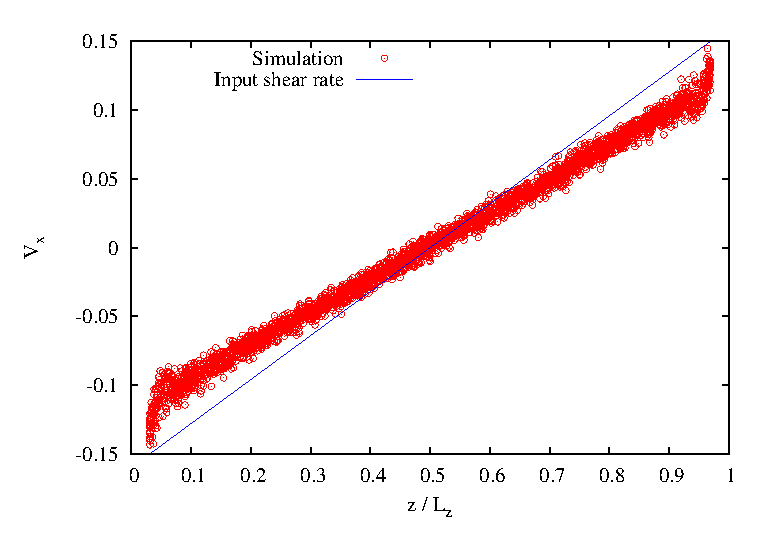
\includegraphics[width=0.7\textwidth]{figs/slip}
\caption{Slip in the simulations for a suspension with concentration $\phi = 0.4$.}
\label{slip_fig}
\end{figure}

\subsubsection{Viscosity from the Irving-Kirkwood Method}

The stress tensor can also be calculated via the Irving-Kirkwood method \cite{irving1950}. Following this method, the stress tensor is calculated from the positions and forces between particles as \cite{bertevas2010,phan2014}:
\begin{eqnarray}
  \boldsymbol{\sigma} &=& \frac{1}{V}\left[\sum_i\boldsymbol{v}_i\boldsymbol{v}_i +
    \frac{1}{2}\sum_i\sum_{j\ne i}\boldsymbol{r}_{ij}\boldsymbol{F}_{ij}\right]
\end{eqnarray}
From the stress tensor, the viscosity can be calculated using Eq. (\ref{eta_from_stress}).

\subsubsection{Comparison of Both Methods}

Results obtained with both methods are compared in this section. The system consists of a suspension with concentration $\phi = 0.4$ in a shear flow between planar walls. Figure \ref{IK_wall_comp} shows the evolution of the ratio $S_{zx}^{\text{wall}} / S_{zx}^{\text{IK}}$ for three different time steps. Although convergence is achieved for $dt = 10^{-4}$ when the stress is calculated from the wall (result not shown here), convergence with the Irving-Kirkwood method requires a time step that is ten times smaller ($dt = 10^{-5}$).

\begin{figure}
\centering
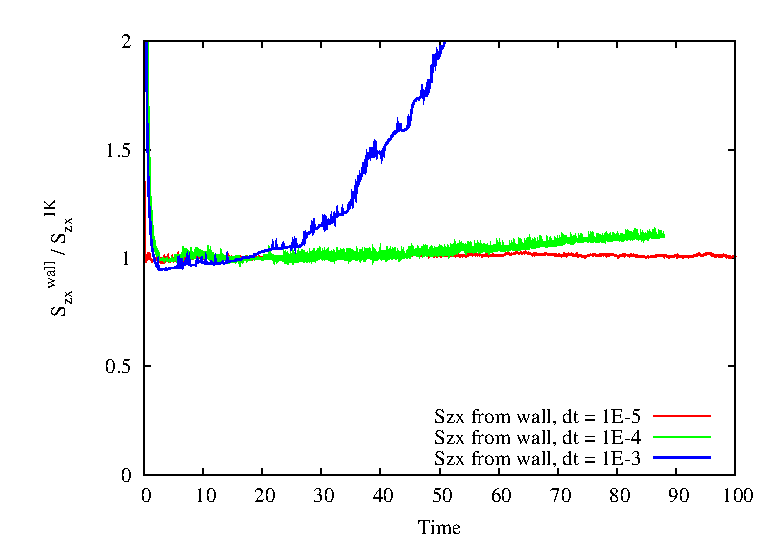
\includegraphics[width=0.7\textwidth]{figs/IK_wall_comp}
\caption{Comparison of the ratio of the component $S_{zx}$ calculated with the wall and the component $S_{zx}$ calculated via the Irving-Kirkwood method.}
\label{IK_wall_comp}
\end{figure}

\subsubsection{Faster Way to Obtain Irving-Kirkwood Results}

It has been observed that the Irving-Kirkwood results for the stress tensor are accurate only for very small time steps. To obtain results more quickly using the Irving-Kirkwood approach, one can run a simulation with a relatively large time step $dt$. Afterwards, in post-processing, the simulation can be continued for a few steps starting from the collected data until the Irving-Kirkwood result reaches a quasi-steady state. Results from such a post-processing calculation have been compared with those from simulations with smaller time steps, showing almost identical results, as depicted in Figure \ref{post_processing_fig}.

To perform the post-processing calculation of the stress tensor, use the script \emph{script\_stress.sh} in the scripts directory.

\begin{figure}
\centering
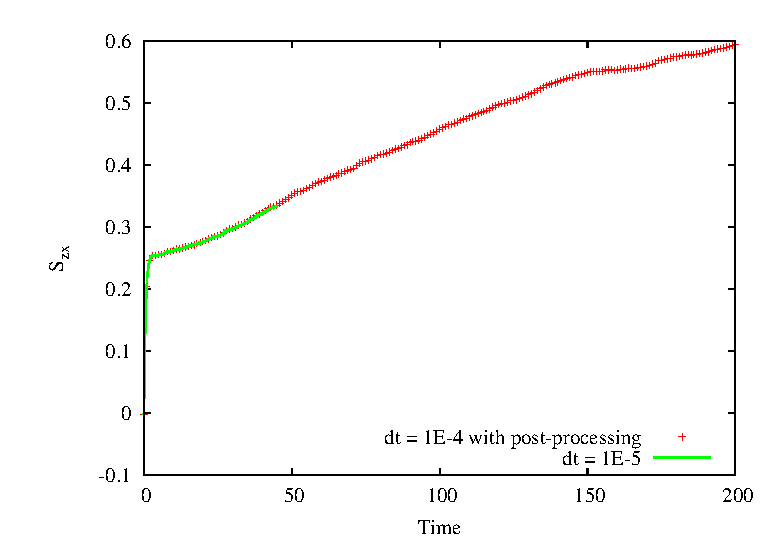
\includegraphics[width=0.7\textwidth]{figs/stress_post_processing}
\caption{Comparison of the temporal evolution of the $S_{zx}$ component of the stress calculated with the proposed post-processing method and another simulation with a smaller time step.}
\label{post_processing_fig}
\end{figure}

\subsubsection{Calculation of the Normal Stress Differences}

The normal stress differences are calculated from the stress tensor as
\begin{eqnarray}
  N_1 &=& \frac{\sigma_{xx} - \sigma_{zz}}{\eta_0 \dot{\gamma}} \nonumber \\
  N_2 &=& \frac{\sigma_{zz} - \sigma_{yy}}{\eta_0 \dot{\gamma}}
\end{eqnarray}

\subsubsection{Viscosity and Normal Stress Differences Versus Concentration}

The dependency of viscosity and normal stress differences on the concentration $\phi$ is shown in Figure \ref{eta_N1_N2}. The normal stress differences are defined as
\begin{eqnarray}
  N_1 &=& \frac{S_{xx} - S_{zz}}{\eta_0 \dot{\gamma}} \nonumber \\
  N_2 &=& \frac{S_{zz} - S_{yy}}{\eta_0 \dot{\gamma}}
\end{eqnarray}
Although the agreement is good for the viscosity of the suspension and for $N_2$, the magnitude of $N_1$ is significantly larger than that obtained by Bertevas et al. It has been verified that the results for $N_1$ and $N_2$ are not sensitive to changes in the cutoff radius and the size of the simulation box (results for $N_1$ and $N_2$ shown in the figures are from a simulation box of size $L = 32 \times 32 \times 32$).

\begin{figure}
\centering
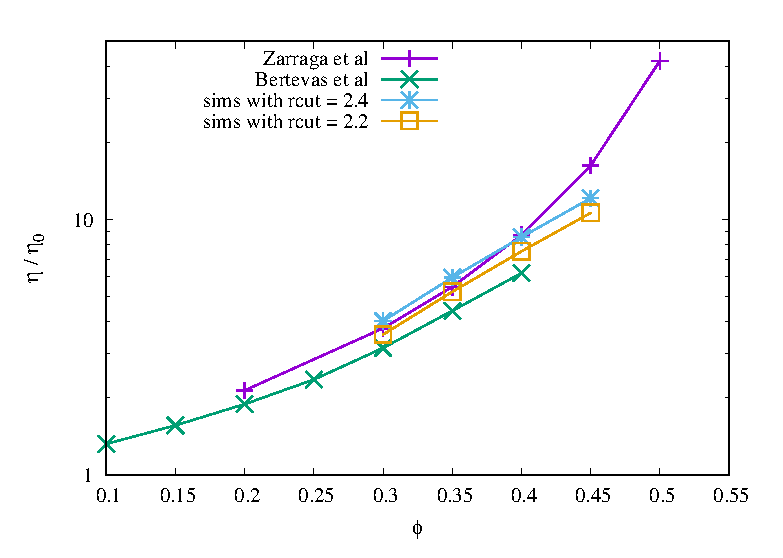
\includegraphics[width=0.7\textwidth]{figs/viscosity_phi}
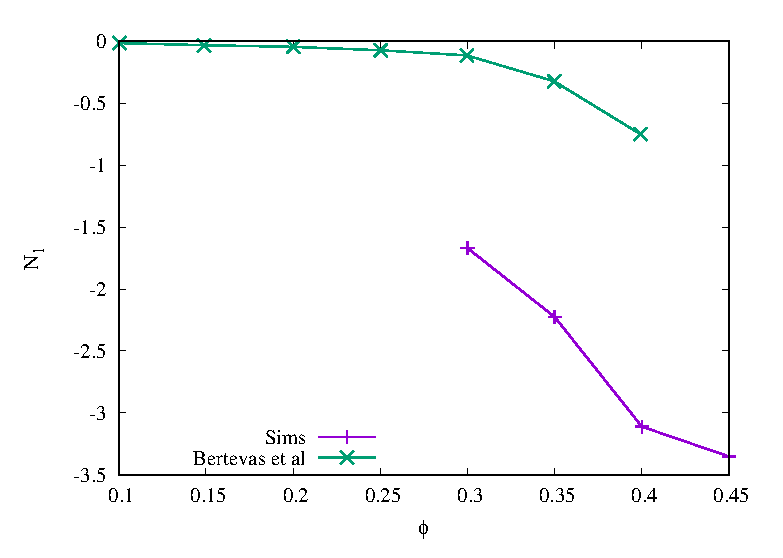
\includegraphics[width=0.7\textwidth]{figs/N1_phi}
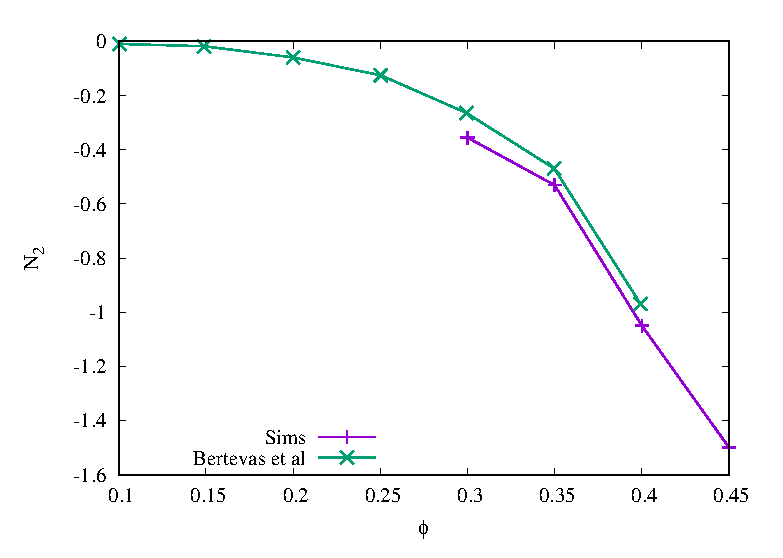
\includegraphics[width=0.7\textwidth]{figs/N2_phi}
\caption{Dependency of viscosity and normal stress differences $N_1$ and $N_2$ on the concentration $\phi$.}
\label{eta_N1_N2}
\end{figure}

%% \section{Some calculations}
%% \subsection{Viscosity calculation}
%% \subsubsection{Viscosity from the wall}
%% Given that the walls are orientated in the $z$ direction, only the components
%% $zx$, $zy$ and $zz$ of the stress can be calculated
%% %
%% \begin{eqnarray}
%%   \sigma_{zx} &=& \frac{F_{wall}^x}{L_xL_y}
%%   \nonumber\\
%%   \sigma_{zy} &=& \frac{F_{wall}^y}{L_xL_y}
%%   \nonumber\\
%%   \sigma_{zz} &=& \frac{F_{wall}^z}{L_xL_y}
%%   \end{eqnarray}

%% The viscosity of the suspension is calculated as
%% %
%% \begin{eqnarray}
%%   \eta &=& \frac{\sigma_{zx}}{\dot{\gamma}}
%%   \label{eta_from_stress}
%% \end{eqnarray}
%% %
%% Note that, in general, the generated shear rate by the wall is not the 
%% input shear rate, given that there is always some slip with the walls
%% (see Fig. \ref{slip_fig}).

%% \begin{figure}
%% \centering
%% 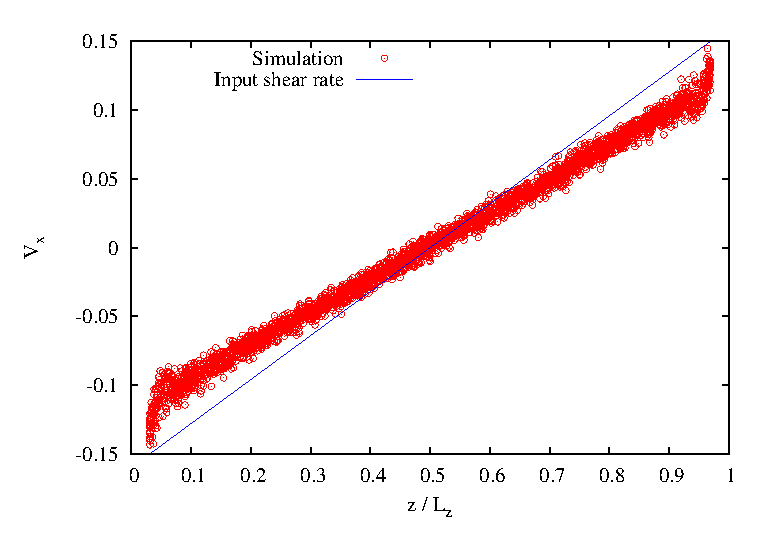
\includegraphics[width=0.7\textwidth, angle = 0]{figs/slip}
%% \caption{Slip in the simulations for a suspension with concentration $\phi = 0.4$.}
%% \label{slip_fig}       % Give a unique label
%% \end{figure}

%% \subsubsection{Viscosity from Irving-Kirkwood method}
%% The  stress tensor  can  also be  calculated  via the  Irving-Kirkwood
%% method \cite{irving1950}. Following this method, the stress tensor can
%% be  calculated from  the  positions and  forces  between particles  as
%% \cite{bertevas2010,phan2014}
%% %
%% \begin{eqnarray}
%%   \boldsymbol{\sigma} &=& \frac{1}{V}\left[\sum_i\boldsymbol{v}_i\boldsymbol{v}_i +
%%     \frac{1}{2}\sum_i\sum_{j\ne i}\boldsymbol{r}_{ij}\boldsymbol{F}_{ij}\right]
%% \end{eqnarray}
%% %
%% From  the   stress  tensor  the   viscosity  can  be   calculated  via
%% Eq. (\ref{eta_from_stress}).

%% \subsubsection{Comparison of both methods}
%% Results obtained with both methods  are compared in this section.  The
%% system consists  on a suspension  of concentration  $\phi = 0.4$  in a
%% shear flow between planar walls. In the figure \ref{IK_wall_comp} the
%% evolution  of  $S_{zx}^{\text{wall}}  / S_{zx}^{\text{IK}}$  has  been
%% drawn for three different time steps. Although the convergence of such
%% a calculation is  achieved already for $dt = 10^{-4}$  when the stress
%% is  calculated  from  the  wall  (result  not  shown  in  here),  when
%% Irving-Kirkwood is used,  the convergence is achieved for  a ten times
%% smaller time step ($dt = 10^{-5}$).

%% \begin{figure}
%% \centering
%% 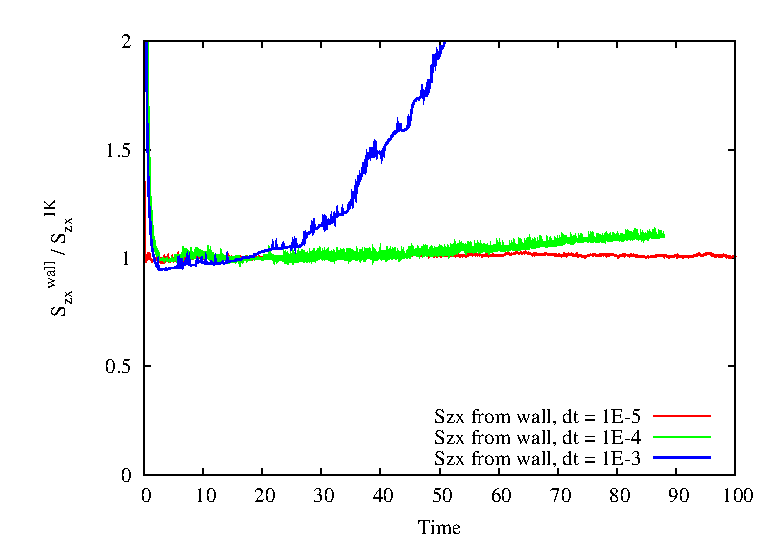
\includegraphics[width=0.7\textwidth, angle = 0]{figs/IK_wall_comp}
%% \caption{Comparison of the ratio of the component $S_{zx}$ calculated
%% with the wall and the component $S_{zx}$ calculated via Irving-Kirkwood.}
%% \label{IK_wall_comp}       % Give a unique label
%% \end{figure}


%% \subsubsection{Faster way to obtain Irving-Kirkwood results}

%% We have  seen that the IK  results for the stress  tensor are accurate
%% only for  very small time  steps. In  order to obtain  results fastest
%% using the IK approach,  we can run a simulation with  a time step $dt$
%% quite  big.   Afterwards,  in  a   post-processing,  we  can  run  the
%% simulation for a  few steps starting from the data  we have collected,
%% until  the IK  result  reaches  a quasi-steady  state. Results with
%% such a postprocessing calculation have been compared to the results
%% from simulations with smaller time steps and both results have been
%% almost identical, as it can be seen in the figure \ref{post_processing_fig}.

%% In order  to do the  postprocessing to calculate  the stress  tensor, the
%% script \emph{script\_stress.sh} in the scripts directory can be used.


%% \begin{figure}
%% \centering
%% 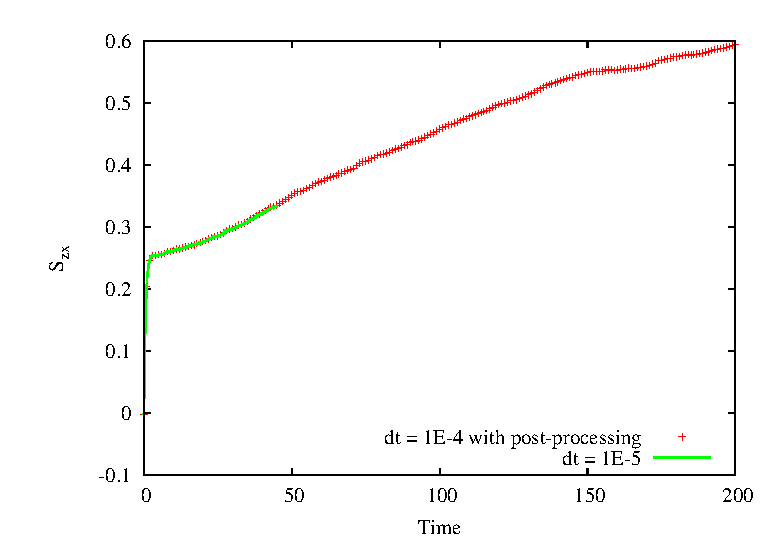
\includegraphics[width=0.7\textwidth, angle = 0]{figs/stress_post_processing}
%% \caption{Comparison of the temporal evolution of the $S_{zx}$ component of the
%%   stress calculated with the proposed post-processing with another
%% simulation with a smaller time step.}
%% \label{post_processing_fig}       % Give a unique label
%% \end{figure}

%% \subsubsection{Calculation of the normal stress differences}
%% The normal stress  differences are calculated
%% from the stress tensor as
%% %
%% \begin{eqnarray}
%%   N_1 &=& \frac{\sigma_{xx} - \sigma_{zz}}{\eta_0 \dot{\gamma}}
%%   \nonumber\\
%%   N_2 &=& \frac{\sigma_{zz} - \sigma_{yy}}{\eta_0 \dot{\gamma}}
%% \end{eqnarray}

%% \subsubsection{Viscosity and normal stress differences
%%   versus concentration}
%% The dependency of the viscosity and the normal stress differences on the
%% concentration $\phi$ have been drawn in the figure \ref{eta_N1_N2}. The normal
%% stress differences are defined as
%% %
%% \begin{eqnarray}
%%   N_1 &=& \frac{S_{xx} - S_{zz}}{\eta_0 \dot{\gamma}}
%%     \nonumber\\
%%     N_2 &=& \frac{S_{zz} - S_{yy}}{\eta_0 \dot{\gamma}} 
%% \end{eqnarray}
%% %
%% Although the agreement is good for the viscosity of the suspension and
%% for $N_2$, the magnitude of $N_1$ is much bigger than the one obtained
%% by Bertevas et al.  It has been  checked that the result for $N_1$ and
%% $N_2$ is not sensitive to changes in the cutoff radius and the size of
%% box of simulation ($N_1$ and $N_2$ from the figures have been obtained
%% with a simulation box of size $L = 32\times 32 \times 32$).


%% \begin{figure}
%% \centering
%% 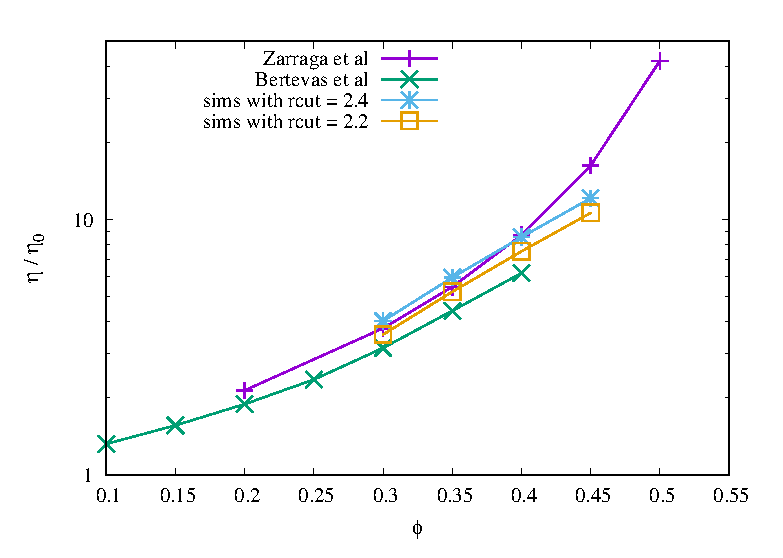
\includegraphics[width=0.7\textwidth, angle = 0]{figs/viscosity_phi}
%% 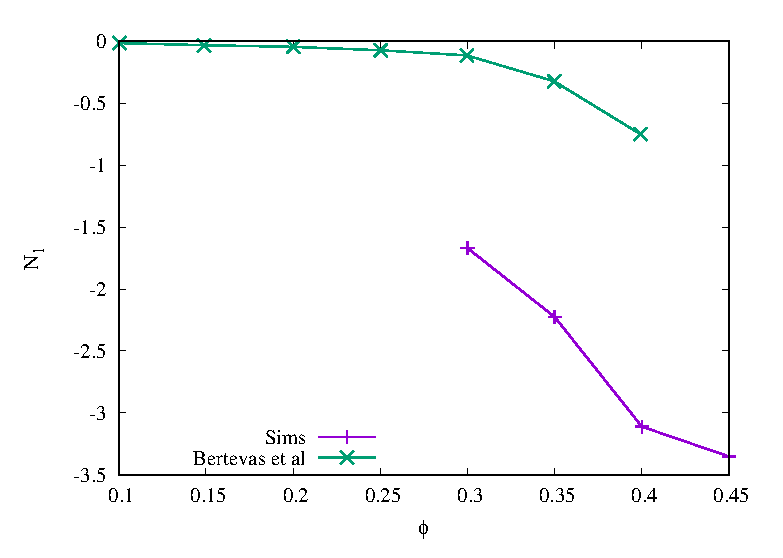
\includegraphics[width=0.7\textwidth, angle = 0]{figs/N1_phi}
%% 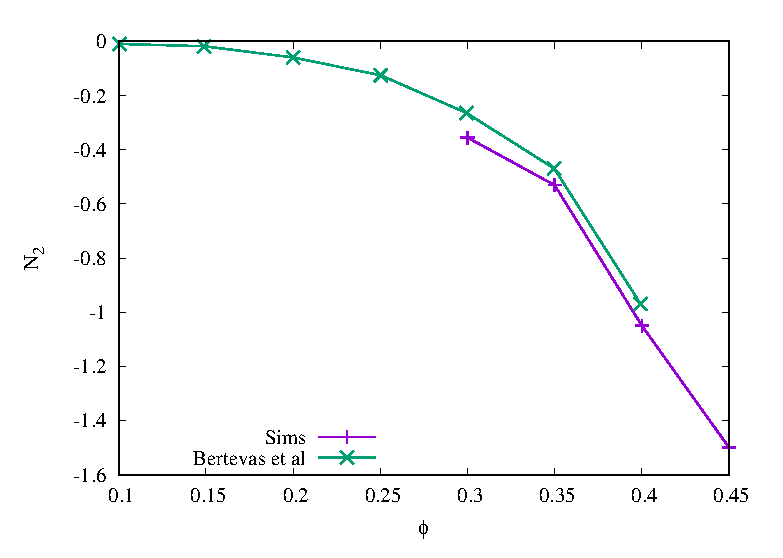
\includegraphics[width=0.7\textwidth, angle = 0]{figs/N2_phi}
%% \caption{Dependency on the concentration $\phi$ of the viscosity and the normal
%%   stress differences $N_1$ and $N_2$.}
%% \label{eta_N1_N2}       % Give a unique label
%% \end{figure}



\bibliography{references}   % name your BibTeX data base
\bibliographystyle{plain}

\end{document}
